%-----------------------------------LICENSE------------------------------------%
%   This file is part of Mathematics-and-Physics.                              %
%                                                                              %
%   Mathematics-and-Physics is free software: you can redistribute it and/or   %
%   modify it under the terms of the GNU General Public License as             %
%   published by the Free Software Foundation, either version 3 of the         %
%   License, or (at your option) any later version.                            %
%                                                                              %
%   Mathematics-and-Physics is distributed in the hope that it will be useful, %
%   but WITHOUT ANY WARRANTY; without even the implied warranty of             %
%   MERCHANTABILITY or FITNESS FOR A PARTICULAR PURPOSE.  See the              %
%   GNU General Public License for more details.                               %
%                                                                              %
%   You should have received a copy of the GNU General Public License along    %
%   with Mathematics-and-Physics.  If not, see <https://www.gnu.org/licenses/>.%
%------------------------------------------------------------------------------%
%   Author:     Ryan Maguire                                                   %
%   Date:       October 24, 2023                                               %
%------------------------------------------------------------------------------%
\documentclass{beamer}
\usepackage{graphicx}
\usepackage{amsmath}
\graphicspath{{../images/}}
\title{Linking Numbers and Causality in Spacetimes}
\subtitle{Knots in Washington $\frac{\sim\texttt{0xF4}}{\texttt{1\;<<\;5}}$}
\author{Ryan Maguire}
\date{December 10, 2023}
\usenavigationsymbolstemplate{}
\setbeamertemplate{footline}[frame number]
\begin{document}
    \maketitle
    \begin{frame}{Outline}
        \begin{itemize}
            \item Spacetimes
            \item Causality and Linking
            \item Linking and Affine Linking Numbers
            \item Gravitational Lensing
        \end{itemize}
    \end{frame}
    \begin{frame}{Spacetimes}
        A Riemannian manifold is a smooth manifold $M$ equipped with a
        \textit{Riemannian metric}, a means of measuring angles between
        tangent vectors that varies smoothly between tangent spaces. That is,
        for each $p\in{M}$ there is a positive-definite symmetric bilinear form
        $g_{p}:T_{p}M\times{T}_{p}M\rightarrow\mathbb{R}$ and for every pair of
        smooth vector fields $X,Y$ the function
        \begin{equation}
            p\mapsto{g}_{p}(X_{p},\,Y_{p})
        \end{equation}
        is smooth.
        \par\hfill\par
        Semi-Riemannian manifolds (also called pseudo-Riemannian manifolds)
        generalize this slightly. The positive-definite condition is relaxed to
        non-degeneracy. For each $p\in{M}$ and for all non-zero $v\in{T}_{p}M$
        there is some tangent vector $w\in{T}_{p}M$ such that
        $g_{p}(v,\,w)\ne{0}$.
    \end{frame}
    \begin{frame}{Spacetimes}
        Sylvester's theorem of inertia tells us that for every $p\in{M}$
        there is a chart $(x_{1},\,\cdots,\,x_{n})$ and three numbers
        $n_{0},\,n_{+},\,n_{-}$ that are constant (independent of the chart)
        such that $n=n_{0}+n_{+}+n_{-}$ and:
        \begin{equation}
            g_{p}=\sum_{k=1}^{n_{+}}\textrm{d}x_{k}^{2}
                -\sum_{k=1}^{n_{-}}\textrm{d}x_{k+n_{+}}^{2}
        \end{equation}
        Non-degeneracy means $n_{0}=0$. The \textit{signature} of a
        semi-Riemannian metric is the ordered pair $(n_{+},n_{-})$.%
        \footnote{%
            Riemannian manifolds have signature $(n,0)$.
        }
    \end{frame}
    \begin{frame}{Spacetimes}
        A \textit{Lorentz} manifold is a semi-Riemannian manifold $(X,\,g)$ of
        dimension $n+1$ with signature $(n,1)$. That is, for every point
        $p\in{X}$ there is a chart $(x_{1},\,\cdots,\,x_{n},\,t)$ such that:
        \begin{equation}
            g_{p}=-\textrm{d}t^{2}+\sum_{k=1}^{n}\textrm{d}x_{k}^{2}
        \end{equation}
        The \textit{null vectors} in $T_{p}M$ are those that satisfy
        $g_{p}(v,\,v)=0$. The equation above tells us that these vectors
        satisfy the equation of a cone.
    \end{frame}
    \begin{frame}{Spacetimes}
        Intuitively, null vectors represent particles traveling at the speed of
        light. We can see this by abusing notation and letting $c=1$. We have:
        \begin{align}
            -c^{2}\textrm{d}t^{2}+\sum_{k=1}^{n}\textrm{d}x_{k}^{2}&=0\\
            \Rightarrow
            \sum_{k=1}^{n}\Big(\frac{\textrm{d}x_{k}}{\textrm{d}t}\Big)^{2}
                &=c^{2}\\
            \Rightarrow
            \sqrt{\sum_{k=1}^{n}\Big(\frac{\textrm{d}x_{k}}{\textrm{d}t}\Big)^{2}}
            &=c
        \end{align}
        This last equation says the \textit{speed} the tangent vector
        represents is equal to $c$, which we're taking to be the speed of light.
    \end{frame}
    \begin{frame}{Spacetimes}
        The \textit{light-cone} at $p$, the set of all null vectors in
        $T_{p}M$, splits $T_{p}M$ into three parts: the interior, the exterior,
        and the cone itself. The interior consists of two connected components.
        \par\hfill\par
        A \textit{time-orientation} is a smooth choice of one of these connected
        components as one varies the point $p$.%
        \footnote{%
            Note: orientable and time-orientable are different. The (open)
            M\"{o}bius strip is not orientable, but it can be time-orientable,
            pending the metric $g$. An annulus is orientable, but it can be
            non-time-orientable, again pending $g$. All four combinations of
            orientable and time-orientable are possible. These are separate
            notions.
        }
        The chosen component is called the \textit{future direction} at the
        point $p$.
        \par\hfill\par
        A spacetime is a Lorentz manifold $(X,\,g)$ with a time orientation.
    \end{frame}
    \begin{frame}{Spacetimes}
        The future and past of a point $p$, denoted $J_{p}^{+}$ and $J_{p}^{-}$,
        respectively, are all points in $X$ that can be connected to $p$ by a
        curve $\gamma$ whose speed is always bounded by the speed of light.
        That is:
        \begin{equation}
            g_{\gamma(t)}(\dot{\gamma}(t),\,\dot{\gamma}(t))\leq{0}
        \end{equation}
        for all $t$.
        \par\hfill\par
        \textit{Nice} spacetimes have the following properties:
        \begin{itemize}
            \item
                $J_{p}^{+}\cap{J}_{q}^{-}$ is compact for all $p,q\in{X}$.
            \item
                No time travel.
        \end{itemize}
        No time travel means there is no future-pointing curve $\gamma$ (not
        exceeding the speed of light) that starts at a point $p$ and later
        returns to $p$.
        \par\hfill\par
        These spacetimes are called \textit{globally hyperbolic}.
    \end{frame}
    \begin{frame}{Spacetimes}
        \begin{theorem}[Geroch, 1970]
            Globally hyperbolic spacetimes $(X,\,g)$ are homeomorphic to
            $M\times\mathbb{R}$ for some topological manifold $M$.
        \end{theorem}
        \begin{theorem}[Bernal-S\'{a}nchez, 2003]
            Globally hyperbolic spacetimes $(X,\,g)$ are diffeomorphic to
            $M\times\mathbb{R}$ for some smooth manifold $M$, and the
            restriction of $g$ to $M\times\{t\}$ can be made Riemannian for all
            $t\in\mathbb{R}$.
        \end{theorem}
        Moreover, $M\times\{t\}$ is a \textit{Cauchy hypersurface},
        a submanifold with the property that particles traveling at
        less-than-or-equal-to the speed of light will intersect $M$ at
        precisely one time moment $t_{0}$.
    \end{frame}
    \begin{frame}{Causality and Linking}
        The \textit{sky} of a point $p$ in a spacetime $(X,\,g)$ is the space
        of all light-rays passing through $p$.
        \par\hfill\par
        If $(X,\,g)$ is globally hyperbolic, the sky of a point $p$ can be given
        a more explicit topological and geometric structure. Let $M$ be a
        Cauchy surface so that $X$ is diffeomorphic to $M\times\mathbb{R}$ and
        let $t_{0}\in\mathbb{R}$ be the unique time such that
        $p\in{M}\times\{t_{0}\}$.
        \par\hfill\par
        Since $(M,\,g|_{M})$ is Riemannian the spherical cotangent bundle
        $ST^{*}M$ can be realized as unit-length elements of $T^{*}M$.
        \par\hfill\par
        For any ray of light $\gamma$ passing through $p$ the linear functional
        $\phi:T_{p}M\rightarrow\mathbb{R}$ defined by:
        \begin{equation}
            \phi(v)=g_{p}\big(v,\,\dot{\gamma}(t_{0})\big)
        \end{equation}
        is non-zero. It hence defines a point in $ST^{*}M$.
    \end{frame}
    \begin{frame}{Causality and Linking}
        The sky of a point can thus be identified with the fibre of $p$ under
        the canonical projection $\textrm{proj}_{M}:ST^{*}M\rightarrow{M}$.
        \par\hfill\par
        The skies of two points $p,q\in{X}$ can be used to answer questions
        about \textit{causality}. That is, whether or not it is possible for
        $p$ and $q$ to communicate with each other by sending messages that
        do not travel faster than light.
        \par\hfill\par
        In some sense the skies of $p$ and $q$ may be \textit{linked} in
        $ST^{*}M$.
    \end{frame}
    \begin{frame}{Causality and Linking}
        $ST^{*}M$ naturally has a contact structure given by the Liouville
        form. One may then ask of the skies of two points are
        \textit{Legendrian linked}, instead of just topologically linked.
        This leads to the following theorem.
        \begin{theorem}[Chernov, Nemirovksi, 2009]
            The skies of causally related points in a globally hyperbolic
            spacetime are Legendrian linked.
        \end{theorem}
        For the remainder of the talk we'll talk about other linking ideas that
        can be used to study causality.
    \end{frame}
    \begin{frame}{Linking and Affine Linking Numbers}
        The linking number of a link with two components can be obtained by
        allowing a component of the link to pass through itself, but not the
        other component. For any two component link you will eventually obtain
        two loops that wrap around each other.
        \begin{figure}
            \centering
            \resizebox{0.65\textwidth}{!}{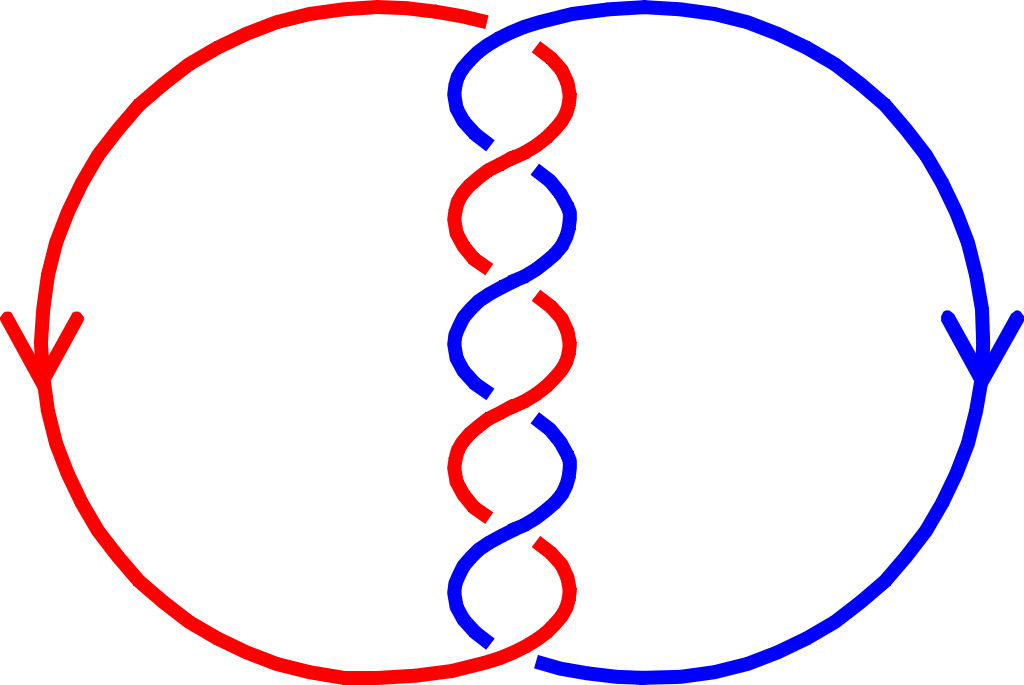
\includegraphics{linking_number_3.png}}
            \caption{Linking-Number Three}
        \end{figure}
    \end{frame}
    \begin{frame}{Linking and Affine Linking Numbers}
        We generalize this to higher dimensional spheres in the spherical
        cotangent bundle of a manifold $M$ via the
        the \textit{affine linking number}.
        \par\hfill\par
        We say that the two spheres $\mathbb{S}_{p}$ and $\mathbb{S}_{q}$ that
        are the fibers of two points $p,q\in{M}$ under the canonical projection
        $\textrm{proj}_{M}:ST^{*}M\rightarrow{M}$ have affine linking number
        zero.
        \par\hfill\par
        Given two arbitrary spheres in $ST^{*}M$ we perturb them until
        we obtain two new spheres that are just the fibers of points $p$ and
        $q$. By keeping track of the number of times a double point occurs
        during this perturbation (and the sign of the double point), we get the
        \textit{affine linking number}.
    \end{frame}
    \begin{frame}{Linking and Affine Linking Numbers}
        For most manifolds, it does not matter how you undergo
        this perturbation.
        \begin{theorem}[Chernov, Rudyak, 2008]
            If $M$ is not an odd-dimensional rational homology sphere, then
            the affine linking number is an invariant.
        \end{theorem}
    \end{frame}
    \begin{frame}{Gravitational Lensing}
        If the curvature of a spacetime is extreme enough, light from one point
        can be seen in various directions and it is possible to see the same
        point multiple times (even infinitely many).
        \par\hfill\par
        This phenomena is known as gravitational lensing. It has been observed
        and well documented by astronomers.
    \end{frame}
    \begin{frame}{Gravitational Lensing}
        \begin{figure}
            \centering
            \resizebox{0.7\textwidth}{!}{%
                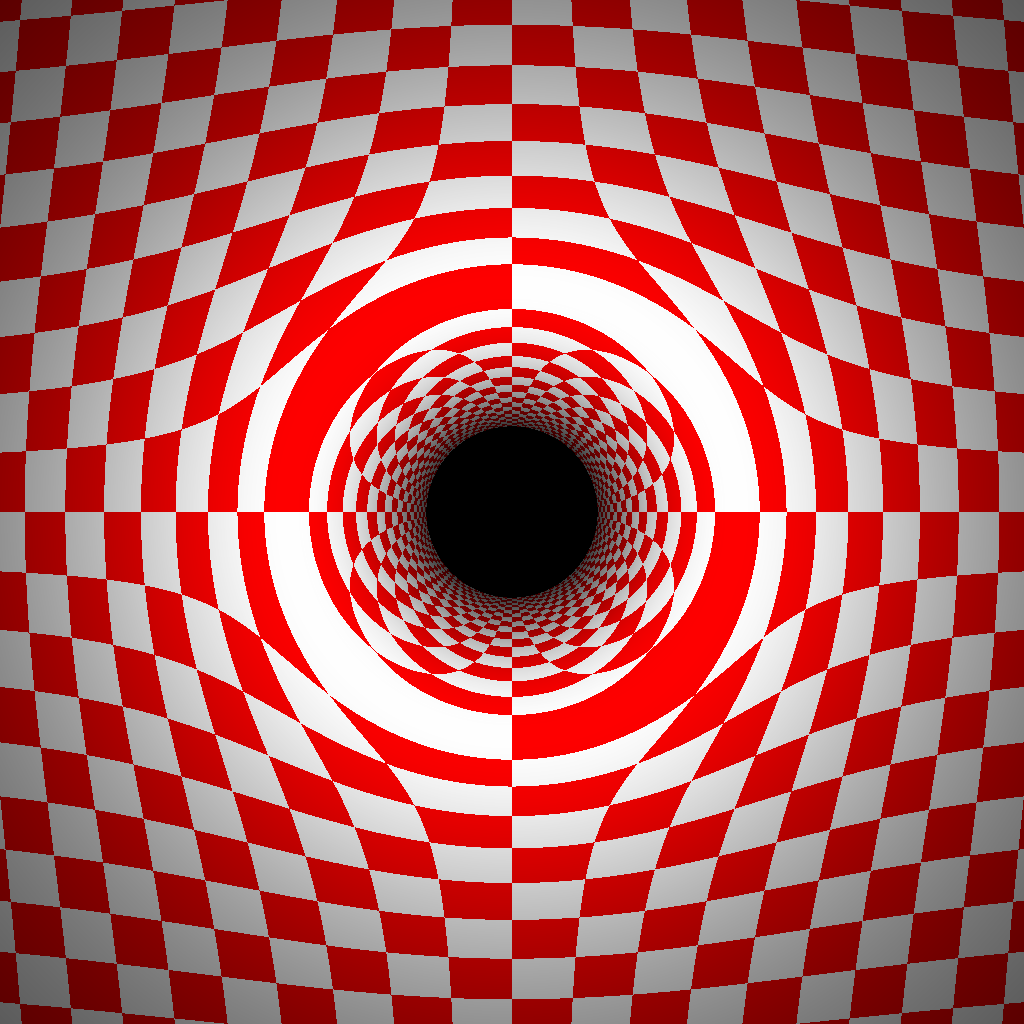
\includegraphics{newtonian_black_hole.png}%
            }
        \end{figure}
    \end{frame}
    \begin{frame}{Gravitational Lensing}
        \begin{figure}
            \centering
            \resizebox{0.7\textwidth}{!}{%
                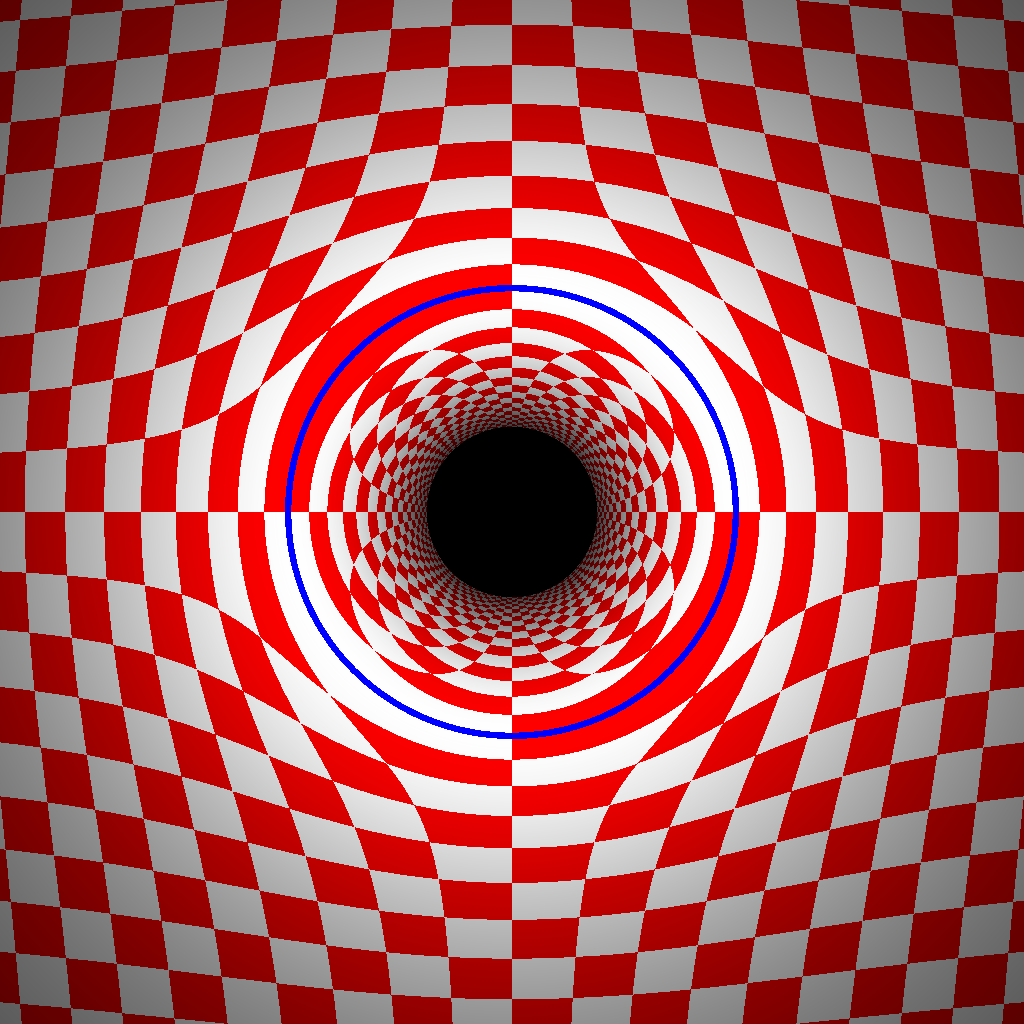
\includegraphics{newtonian_black_hole_center_highlight.png}%
            }
        \end{figure}
    \end{frame}
    \begin{frame}{Gravitational Lensing}
        \begin{figure}
            \centering
            \resizebox{0.7\textwidth}{!}{%
                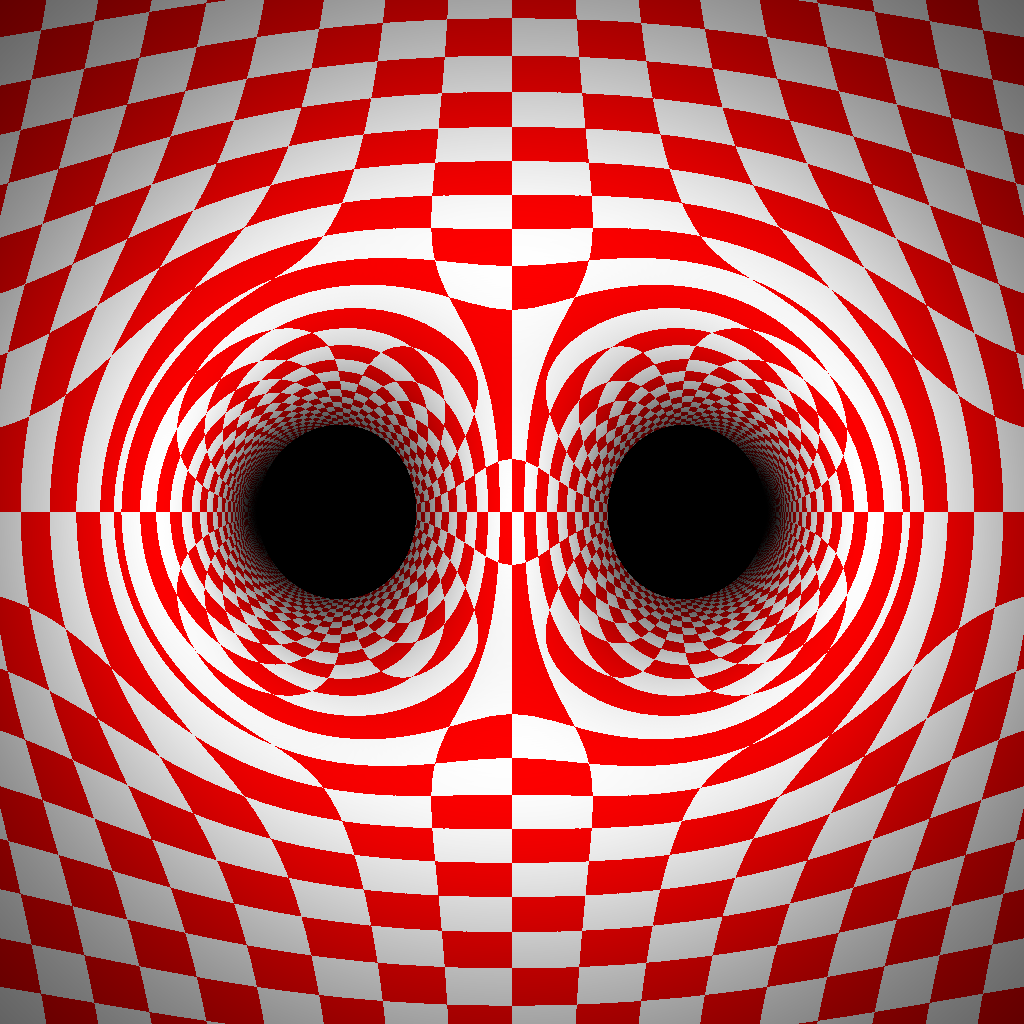
\includegraphics{newtonian_black_hole_two.png}%
            }
        \end{figure}
    \end{frame}
    \begin{frame}{Gravitational Lensing}
        \begin{figure}
            \centering
            \resizebox{0.7\textwidth}{!}{%
                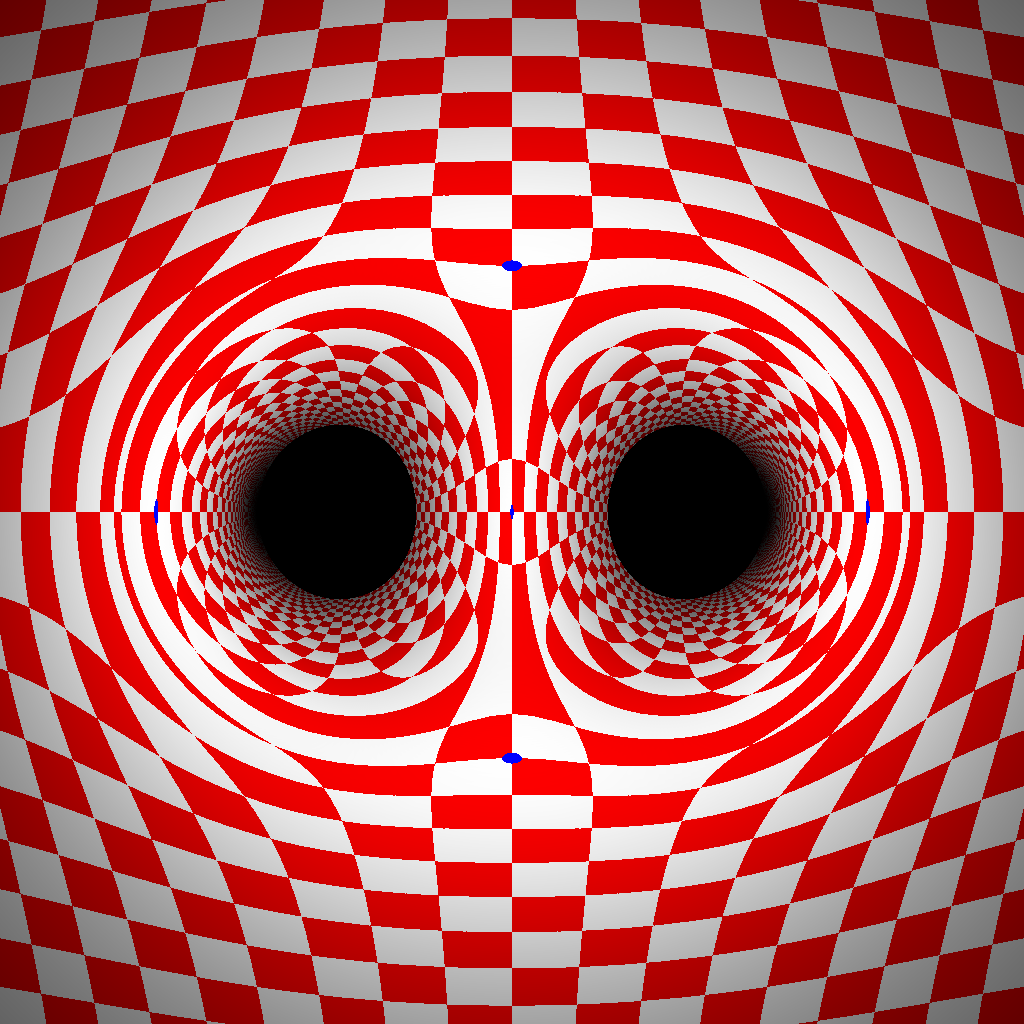
\includegraphics{newtonian_black_hole_two_center_highlight.png}%
            }
        \end{figure}
    \end{frame}
    \begin{frame}{Gravitational Lensing}
        \begin{figure}
            \centering
            \resizebox{0.7\textwidth}{!}{%
                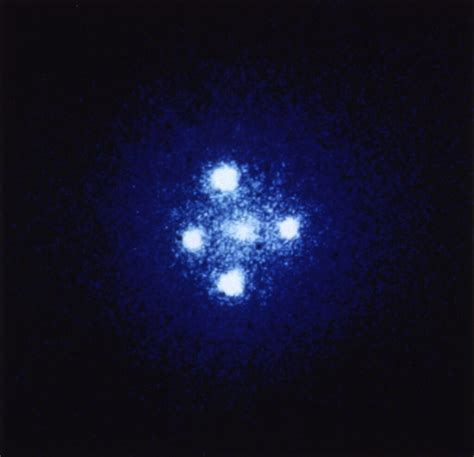
\includegraphics{einstein_cross_001.png}%
            }
        \end{figure}
    \end{frame}
    \begin{frame}{Gravitational Lensing}
        Affine linking number can be used to detect how many times an observer
        sees a given point.
        \begin{theorem}[Chernov, Maguire, 2023]
            Assume $(X, g)$ is globally hyperbolic and the Cauchy surface
            of it is not an odd dimensional rational homology sphere.
            Let $\gamma:(-\varepsilon,\,\varepsilon)\rightarrow{X}$
            be a small timelike curve that passes through $p$ at time moment 0.
            If:
            \begin{equation}
                \textrm{alk}(\mathbb{S}_{\gamma(\varepsilon)}, \mathbb{S}_{q})-
                \textrm{alk}(\mathbb{S}_{\gamma(-\varepsilon)}, \mathbb{S}_{q})
                =N
            \end{equation}
            for all small $\varepsilon$, then the observer at $p$ sees light
            from $q$ coming from at least $N$ different directions.
        \end{theorem}
        If the time-like sectional curvatures of $X$ are non-negative, this
        becomes sharp. The observer at $p$ sees \textit{exactly} $N$ copies of
        the point $q$.
    \end{frame}
    \begin{frame}
        \begin{center}
            Thank You!
        \end{center}
    \end{frame}
\end{document}
